% Bachelor Thesis, 2012
% Software Engineering at Blekinge Institute of Technology
% 
%
% Authors:    Fredrik Olsson, Johannes Björk
% Supervisor: Nina D. Fogelström
% 
% Copyright 2012,  Fredrik Olsson and Johannes Björk
% All rights reserved

\documentclass{llncs}

\usepackage[utf8x]{inputenc}
\usepackage{pdfpages}
\usepackage{graphicx}
\usepackage{ctable}
\usepackage{tabularx}
\usepackage{subfig}

\title{Overcoming the initial obstacles with Enterprise Service Bus}
\author{Johannes Björk \inst{1} \and Fredrik Olsson \inst{1}}

\institute{
	Blekinge Institute of Technology \\
	\email{johannes@johannesbjork.se}, \email{spooky.bender@gmail.com}
}

\hyphenation{ESB foo-bar-baz}

\begin{document}

\maketitle

\begin{abstract}
As 

\keywords{ESB, Enterprise Service Bus}
\end{abstract}

\newpage
\setcounter{tocdepth}{3}
\newpage

\section{Introduction}
A lot of companies have an increasing need to integrate different software to create systems that is able to automatically handle large parts of business logic. Systems that are integrated with each other can save both time and money, as they can cut out time consuming, manual handling of data transfer.

The current de facto standard for software integration is called Enterprise Service Bus (ESB). The ESB handles all communication between different individual systems (nodes) that are to be integrated in the finished system.

The ESB needs to be able to provide different interfaces for nodes to communicate and also needs the capability to transform data so that all nodes receives data that it can understand and work with.

But how easy is it to start up with integration using an ESB?

The goal of this paper is to find a majority of all the known issues with software integration with Enterprise Service Bus (ESB), and also try to find solutions to these issues.

The purpose is to make integration with ESB easier by pinpointing the available solutions to known issues and if no solutions are available, try to find our own methods to deal with problems.

The aim is to provide some kind of solution to every issue that we encounter during the literature review section.

Our methods consist of two parts:
\begin{enumerate}
 \item Literature review - Information will be collected from research databases available via BTH and the collected articles will give a base of issues that needs to be addressed.
 \item Interviews/Surveys - Based on the result from the literature review, a survey will be created where we will try to confirm if our found issues are also experienced by the practitioners. If so, do they have a possible solution of their own and if not, how are the issues handled.
\end{enumerate}
The result of this paper will hopefully provide a guideline to developers that are new to integration with ESB. A resource that will help them get past the most common issues and give them a quicker start with development.


\section{Background}
In this section we will provide the background knowledge that can be usefull to be able to understand what we are really talking about.
The techniques and terms explained are:
\begin{itemize}
\item Point-to-Point Integration
\item Hub-and-Spoke Integration
\item Enterprise Servise Bus (ESB)
\item Service Oriented Architecture (SOA)
\item Simple Object Access Protocol (SOAP)
\item Web Services Description Language (WSDL)
\item Universal Descriptionm Discovery and Integration (UDDI)
\item Representational State Transfer (REST)
\item Client-server
\item Stateless
\item Cache
\item Uniform interface
\item Layered system
\item Code-on-demand
\item a description of our current software engineering project
\end{itemize}

\label{sec:background}

\subsection{Point-to-Point Integration}
Our existing integration architecture is the result of the Point-to-Point integration pattern. Initially not much thought was given to the integration because of software development was mostly done on a application level. Most of the communication was an internal one. While this method of integration was done quickly and cheaply it became very hard and expensive to expand if new connectivity was required. Today's integration problem as a result of tightly fitted software coupling could be traced back to this early integration pattern. The topology makes it very hard add a node into this integration pattern. Because every node in the web needs to have connectivity with each other, increases each additional node the complexity of the system. The  formula for calculating the number of connection for each additional node is (n(n-1))/2 where n is the number of nodes that needs to be integrated. For example if 5 nodes needs to be integrated 10 individual connections are required.

This method is simple and may appeal when there is just a few nodes that needs to be integrated but when the business changes and there is a need to add additional nodes the integration may become extremely costly and the result very brittle. If your application just contains 3 nodes or less and no plans for further expansion is likely. Then Point-to-Point is possibly a good solutions to use but otherwise a more complex integration pattern should be considered.


\subsection{Hub-and-Spoke Integration}
The Hub-and-Spoke method is the next step of integration patterns. In this method a central hub connects each node with a spoke. For each additional node added to this pattern only a single new connection needs to be created. From this model much of the required components that exists today was laid out here: Message transformation, Message protocol standards, protocol security translation and so on. Once integration with multiple system was possible the need to share resource became great. The first method of integration with multiple systems came with the Remote Procedure Call (RPC) which was designed to function in a similar way as a local procedure call would. The rise of distributed computing required a more modular system architecture and as a result required a more complex integration solution. The technologies of Remote procedure call and Distributed Object uses a method of tightly specified interfaces. As the system became more complex the and more changes to the interfaces as a result, it became very hard and costly to maintain and update those interfaces. Additional problems was that disparate system was not able to natively communicate with each other and resulted with many communication problems. These problems resulted in the rise of manny communication technologies. One of those was Web Services which is a point-to-point with well defined interfaces and loosely coupled. The definition of loosely coupled is that the message can contain an undefined payload in either a text or a binary format.

The advantages of hub and spoke compared to point to point is that it has a reduced number of required connections. It also decouples the different nodes so they do not have to know about each other and makes it much easier to add and remove nodes. Because the only changes that have to be made is in the hub. As a result we have a system of independent distributed nodes that are interchangeable and easy to scale when new nodes have to be added.

\subsection{Enterprise Service Bus ESB}
The Enterprise Service Bus is the newest iteration of Integration solutions. The topology resembles that of the Hub-and-Spoke. The main difference of the ESB to the Hub-and-spoke is that ESB focus on open standards and manly on Service Oriented Architecture.

Some of the core features of an ESB:
\begin{itemize}
\item Message transformation - To transform messages between different message protocols.
\item Message Enrichment - the ability to enrich required missing data into a message.
\item Message Routing - A message should be able to traverse the flow in number of ways according to standard patterns.
\item Protocol translation - The possibility to send message on different types of transmission protocols.
\item Security - To be able to translate and support different security protocols.
\item Messaging- Support for asynchronous and synchronous messaging, request/response, send-and-forget, publish/subscribe.
\item Transaction Management - The ability to support different types of transaction standards.
\item Platform independent - The ESB should only use protocols and technologies that are platform independent.
\item Audit - Monitoring status, logging, metrics, admin console.
\item Legacy System - Support for legacy system protocols to allow integration with older system.
\item Message Aggregation/Splitting - To be able to merge and split messages.
\item Schema Validation - The possibility to verify the correctness of a message according to the message definition.
\item Business rules - To support integration with a Business processing language.
\end{itemize}



\subsection{Service Oriented Architecture SOA}
SOA is a framework for integration based on open defined standards. It focuses on services with  loosely coupled well defined interfaces. As it uses platform independent standards it is a good fit for integration in heterogeneous environments. SOA exposes a well defined interface for service and uses stateless implementations to perform specific business tasks. The standards which SOA achieves its platform independence is Simple Object Access Protocol (SOAP) which is a message protocol defined in xml, Web Service Description Language (WSDL) which is a definition of what a SOAP message should contain and which SOAP operations exists, the Universal Description, Definition and Integration (UDDI) which contains which services a system exposes, Representational State Transfer (REST) is constraints which message and process should behave and WS-I which is guidlines to make disparate system interoperable.

\subsection{Simple Object Access Protocol SOAP}
SOAP is a XML based message protocol. It can be together with other application layer protocol but are mostly sent with HTTP. SOAP is platform independent and therefore much used for software  integration. SOAP is the next generation XML-RPC but it still borrows some of its features. SOAP can be combined with WS-* standards like WS-Security which adds a layer of security to the protocol, by requiring username and password or other types of security tokens. The SOAP protocol has some advantages/disadvantages.

Advantages
\begin{itemize}
\item The SOAP protocol allows transportation on a various un specific types of application and transportation layer protocols.
\end{itemize}
Disadvantages
\begin{itemize}
\item The protocol can be considered slow because of its XML format with its verbose nature is easy for humans to read but unnecessary large for a computer to process. Small messages can result in performance issues because of the large XML overhead that is required in SOAP. There is alternatives to SOAP where data is sent in binary form it reduces the size but makes it harder to correct errors.
\end{itemize}


\subsection{Web Services Description Language WSDL}
WSDL is a XML based schema languages used to define which operations a web service provides. It provides detailed information of what the message shall contain, which data types the data shall be in, what operation shall be performed, which URL the request shall be sent to, what a successful and error message should look like and contain. WSDL works well with SOAP. The WSDL is published together with the service so that a SOAP message can be generated to whoever has access to the service. Additionally a incoming SOAP message can be validated according to the WSDL so that only messages that follows the standard will be processed. This feature can be expensive so it is usually turned off when the communication is internal because it relies on that the connecting client follows the standard without having to verify it.

\subsection{Universal Description, Discovery and Integration UDDI}
UDDI is a XML standard that contains information about Web Service and its functionality. it uses SOAP to communicate. It is used for identify what a service does and help a consumer find which service suits him best to perform a specific task. The register also contains technical information and links to the various WSDL.

\subsection{Representational state transfer REST}
REST is a standard for how a web standard like HTTP and URL should be used. To confirm to this standards is to be RESTful. The REST architecture have six constraints.

\subsubsection{Client–Server}
Separating user interface with data storage. The server is not aware of the user interface it just provides the data and vice versa. This will improve the scalability allowing the clients to be interchangeable.

\subsubsection{Stateless}
No client context should be stored on the server. Every request should contain all the required information. Session state should therefore be held on the client. This method will increase the scalability because of no context data will be required to shared over the system. There is also disadvantages like increased data transmission because of no data will be stored on the server. Resulting in repetitive data transmission of the user credentials.

\subsubsection{Cache}
Having support for labeling message cacheable or uncacheable. Allowing the client  to reuse response data later. Advantages of this method is that the response for request will be reduced. Disadvantages of this is that caching allows the possibility of the data becoming stale.

\subsubsection{Uniform Interface}
Decoupling the interface from the service allowing the client and server application to be developed  independently. The disadvantage is that the data need to be transformed into a general form before being transmitted instead of being in the form of what an specific application optimally wants it in.

\subsubsection{Layered System}
Using a architecture hierarchy will result in improved system scalability, allowing load-balancing and shared caches. The client will not know if he is connected directly to the server or to a intermediary like a load balancer. This layer system style shields each layer so that each component just sees the component it communicates with. This allows the component layers to be interchangeable.

\subsubsection{Code-on-Demand}
This is an optional constraint. This allows the server to provide finished code that contains general functionality to be used in client. Allowing the server to change part of the client code. The code can be in a form of JavaScript or Java applets.

\subsection{Student project}
We are currently involved in a student project together with 10 other student that works together with Ericsson. The goal of this project is to integrate several of Ericssons existing products to create a totaly new system. There is a lot of things that we are not allowed to mention about this project but the technique of choise for integration is no secred, we are using a ESB solution by Mulesoft. Because of this, a lot of information and experience can be collected from the participants in this project.



\section{Research questions and research design}
In this section we will present our research questions and also how we plan to find answers to these questions. We will provide the details on how we will collecte published articles and how this will lead to the forming of a questionare to be used in further information gathering.
\subsubsection{Research Questions}

\begin{description}
\item[RQ1] What disadvantages are mentioned of ESB solutions and in what context in the literature?
\item[RQ2] What disadvantages are experienced by the practitioners?
\item[RQ2.1] Are there any available suggested solutions or improvements?
\end{description}

\subsection{Methods for answering research questions}

\begin{description}
\item[RQ1] Study of the result from the literature review.
\item[RQ2] Interviews with participants from Ericsson and also developers from the project we are currently working in. The interviews will be conducted with a survey based on the result from \emph{RQ1}.
\item[RQ2.1] Study of the result from \emph{RQ1} and answers given in \emph{RQ2}. Besides this, we will gather information from the various communities connected to the different ESB solutions.
\end{description}

\subsection{Literature review design}
Information has been gathered from research databases using the following query strings:
\begin{itemize}
\item enterprise service bus
\item esb problems
\item esb issues
\item enterprise service bus problems
\item enterprise service bus issues
\item esb advantages
\item esb disadvantages
\item enterprise service bus advantages
\item enterprise service bus disadvantages
\end{itemize}

Searches were conducted on the library of Blekinge institute of technology and our preferred databases are \emph{Engineering Village} and \emph{IEEE}.

To limit our results, we decided to disregard articles that were published prior to 2005, as this field is in eternal progress and information gets old fast.
Other criteria that needs to be met is a clear value to the purposes of this paper in the abstract, since time is of the essence we will not have time to read papers that we are not sure will give 

\subsection{Interview survey design}

We will conduct interviews with participants in our development team that are currently in the process of implementing an ESB with the help of a survey and also with developers from Ericsson. The survey is created from the result of the literature review and is designed to accomplish two things.
\begin{enumerate}
\item Confirm that the known issues from the literature review is also present in the projects we are involved in. If this is not the case, show how the particular issue has been handled.
\item See if there are other issues that we have not found in previous research papers. We will also try to get the participants to try to think of possible solutions.
\end{enumerate}
Our goal is to have a range between six to eight participants in this survey with varying experience in ESB Integration. We initially try to get as many professional ESB Integrators as possible then if they are not enough we will ask participants from our software project who has experience in ESB integration. The reason we decided on the number of participants was because of the limited time we had we thought it reasonable with that range of people. The challenge was to find people we the experience who also had time to spare to answer our questionnaire. 

The survey will contain the following questions and might be followed up by additional questions:
\label{survey}
\begin{itemize}

\item Do you have any experience with software integrating using an ESB?
\begin{itemize}
\item If so, what?
\end{itemize}

\item Is it hard to decide which part of the system functionality really belongs in the ESB?
\begin{itemize}
\item If so, please elaborate
\item If not, how do you decide?
\end{itemize}

\item Do you experience an issue with slower communication between nodes because of the extra steps that comes with an ESB?
\begin{itemize}
\item If so, please elaborate
\item If not, is it because the steps do not take any time or because the system does not require response?
\end{itemize}

\item Have you ever migrated older, integrated systems to the ESB architecture?
\begin{itemize}
\item If so, please describe the main issues encountered.
\item How did you do to resolve said issues?
\end{itemize}

\item Are you able to get support or find information to resolve the issues that are encountered during integration?
\begin{itemize}
\item If so, how do you find/get said help?
\item If not, how do you handle issues?
\end{itemize}

\item Have you encountered any issues, apart from the ones mentioned in this questionnaire, when working with ESB integration?

\item Have you been able to resolve any of these issues?
\begin{itemize}
\item If so, please describe your solutions.
\end{itemize}

\end{itemize}

\subsection{Literature review results}

The following papers were found during our literature review, and passed our selection criteria:
\begin{enumerate}
\item Enterprise Service Bus: A Performance Evaluation\cite{sanjay11}. Published by Sanjay P. Ahuja, Amit Patel in 2011. This paper seemed useful because it contained a performance analysis between different types of ESBs.
\item SOAs \& ESBs\cite{paisley05}. Published by J. Paisley in 2005. This article brings up some of the difficulties that can be encountered when implementing an ESB.
\item Getting on Board the Enterprise Service\cite{ortiz07}. Published by S. Ortiz in 2007. This article brings up some of the challenges that can be encountered when implementing an ESB.
\item A high performance enterprise service bus platform for complex event processing\cite{bo08}. Published by Deng Bo,  Ding Kun and Zhang Xiaoyi in 2008. This paper brings up some of the challenges that can be encountered when implementing a complex ESB solution.
\item Service-Oriented Performance Modeling the MULE Enterprise Service Bus (ESB) Loan Broker Application\cite{brebner09}. Published by P. Brebner in 2009. This paper handles both scaling and performance in ESBs.
\item An integration strategy for large enterprises\cite{risimic06}. Published by Dejan Rismic in 2006. It provides information on important aspects of ESB. This is needed to be able to understand and improve the ESB.
\item Performance Prediction of Service-Oriented Applications based on an Enterprise Service Bus\cite{gorton07}. Published by Yan Liu, Ian Gorton and Liming Zhu in 2007. This paper handles important aspects of ESB performance. Needed to be able to find performance issues.
\end{enumerate}

After we settled on the these specific documents, we began reading through them from top to bottom, noting everything that can be seen as an issue or flaw in the ESB architecture.
Some of the included documents is not part of the literature to provide a source of issues, but instead serves as a source to be able to get better understanding of the ESB.
Besides these, all documents have one common denominator: They handle aspects of the ESB that can be seen as issues or in need of improvement.
The literature study gave us the following list with issues/flaws in ESB solutions:

\begin{enumerate}
\item It is hard to decide where all functionality goes. Some things could be placed in the ESB but might as well be in one of the nodes in the system \cite{ortiz07}.
\item There is a risk of slow performance, as the ESB prohibits direct communication between nodes.
\item Migration of systems integrated with older architectures can be hard to do \cite{ortiz07}.
\item Support is sometimes limited and documentation and community answers is not always available without a lot of effort.
\end{enumerate}

We thought that we would find more issues in this field and there is a slight possibility that we have missed articles that could provide more information. But we feel confident that the search strings we used, in the databases we searched, provided us with articles that together covers the issues that are involved with integration with an ESB architecture.

\section{Data collecting results}
In this section we will present the results we got from the sampling that we performed.
\subsection{Survey setup}

Our survey where filled out by seven individuals, all in some way connected to our current project at Ericsson. We chose participants based on their previous knowledge of system integration. Both with ESB and other techniques. Four of the participants are in our group and are currently working actively with integration using a ESB from Mulesoft. The other three are employees at Ericsson, which we have got in contact with while performing our project at Ericsson.
The surveys was conducted by handing the participant a printed survey with our previously stated questions  in section \ref{survey}. After this, the person had all the time he or she needed to fill in their answers.
All the participants had one of us present at all time in case something was unclear, badly formulated or in case they just wanted to say something that was not covered by the survey. The survy where done anonymously by all participants. Their roles and experience where recorded during the interviews. The information can be found in Apendix A.

\subsection{Collected data}
The collected answers from the survey can be found in appendix A.

\subsection{Data analysis}

To map our results to our research questions, we begin by rereading the issues we found in the literature review:

\begin{enumerate}
\item It is hard to decide where all functionality goes. Some things could be placed in the ESB but might as well be in one of the nodes in the system.
\item There is a risk of slow performance, as the ESB prohibits direct communication between nodes.
\item Migration of systems integrated with older architectures can be hard to do.
\item Support is sometimes limited and documentation and community answers is not always available without a lot of effort.
\end{enumerate}

If we compare these initial issues one by one with the answers we got, we will see how well it maps with the development process, this may also provide a solution to the initial issues. This will later lead the way to an answer on research question 2 and 2.1

\begin{tabular}{ | l | p{9cm} | l | l |}
\hline
Nr & Question & Yes & No \\ \hline
Q1 & Do you have any experience withintegration using a ESB? & 7 (100\%) & 0 (0\%) \\ \hline
\end{tabular}

\begin{description}
\item[Q1] The first question was an open ended question where the interviewee would describe their experience developing integration solutions using an ESB. To get a feel on how trustworthy and reliable their answers would be.
\end{description}

\begin{tabular}{ | l | p{9cm} | l | l |}
\hline
Nr & Question & Yes & No \\ \hline
Q2 & Is it hard to decide which part of the system functionality really belongs in the ESB? & 4 (50\%) & 4 (50\%)\\ \hline
\end{tabular}

\begin{description}
\item[Q2] On this question, we get a 50\% distribution of agreement to this issue. This is due to one participant answering “yes and no”. As it is not a unanimous agreement that the initial issue is in fact an obstacle, this provides possible solutions to the issue in question.
\end{description}

\begin{quote}
  quote
\end{quote}

\begin{tabular}{ | l | p{9cm} | l | l |}
\hline
Nr & Question & Yes & No \\ \hline
Q3 & Do you experience an issue with slower communication between nodes because of the extra steps that comes with a ESB? & 2 (29\%) & 5 (71\%) \\ \hline
\end{tabular}

\begin{description}
\item[Q3] When trying to confirm this issue, we got ~71.4\% disagreement from the partitioners in the survey. As this is quite a large percentage it indicates that this is not a major issue. But still it’s not 100\%, so there may still be ways to resolve it.
\end{description}

\begin{tabular}{ | l | p{9cm} | l | l |}
\hline
Nr & Question & Yes & No \\ \hline
Q4 & Have you ever migrated older, integrated systems to the ESB architecture? & 0 (\%) & 7 (100\%) \\ \hline
\end{tabular}

\begin{description}
\item[Q4]  Unfortunately we couldn’t find anyone who had dealt with migration of older integrated systems to the ESB architecture. This prevents us from obtaining solutions to issues connected to this issue.
\end{description}

\begin{tabular}{ | l | p{9cm} | l | l |}
\hline
Nr & Question & Yes & No\\ \hline
Q5 & Are you able to get support or find information to resolve the issues thatare encountered during integration? & 6 (86\%) & 2 (14\%)\\ \hline
\end{tabular}

\begin{description}
\item[Q5] This is clearly an issue in the industri. ~86\% of the participants in our servey claim to have problem in finding the information and support they need. The remaining percentile said when asked, that he had not been that involved with integration that he had to find any information that wasn't already available within the group.
\end{description}

These results provides us with possible answers to both research question 2 and 2.1 on all points except the issue with migration of previously integrated systems.

Since research question 1 gets its answers through the literature survey, this is a satisfiable result.

\section{Data synthesis and answer to research questions}
We found possible solutions to the majority of the known issues we found, these solutions are not guaranteed to work for everyone and in any situation but it still may provide assistance for developers that are stuck in the process of either deciding on integration architecture or are in active development.
From the survey we also got some additional issues concerning ESB integration that was not found in the available literature, some of these issues came with a solution and some came with hints on how to find a solution.

\subsection{Results}

\begin{description}

\item[RQ1] The following issues can occur when implementing an ESB architecture solution in a software project (according to available documentation):
\begin{description}
\item[1.1] It is hard to decide where all functionality goes. Some things could be placed in the ESB but might as well be in one of the nodes in the system.
\item[1.2] There is a risk of slow performance, as the ESB prohibits direct communication between nodes.
\item[1.3] Migration of systems integrated with older architectures can be hard to do.
\item[1.4] Support is sometimes limited and documentation and community answers is not always available without a lot of effort.
\end{description}

\item[RQ2] The following issues were presented during the survey in addition to the issues found in the literature review:
\begin{description}
\item[2.1] If the team developing the ESB falls behind, this affects all teams that utilize the ESB.
\item[2.2] Big changes between different versions of the ESB makes it hard when documentation isn't up to date.
\item[2.3] There is no stated standard, or best practise, when it comes to ESB implementation.
\item[2.4] Problems when different nodes use different sessions. The ESB is usually stateless, meaning that it has no session id, this can be a problem if some nodes need their own sessions.
\item[2.5] A lot of the ESB coding is done in XML which is not a proper programming language and this makes it hard to get a good overview of the code. 
\item[2.6] To get proper documentation, a enterprise license might be needed. This is expensive and might raise the projects budget.
\end{description}

\item[RQ2.1] The provided, possible solutions to the encountered issues:
\begin{description}
\item[1.1] In real world implementation, it is important to set rules of communication. As can be seen in the answers to question 2.2 in appendix a, a firm rule of how communication needs to be applied when beginning ESB implementation. 
\item[1.2] This should not be an issue as the ESB only performs actions that would need to be done by the individual nodes if the ESB wasn’t there to sort it out. As long as the ESB only does what it needs to do, all nodes should get what it needs, when it needs it. Any bottlenecks is most likely to be found in connection or slow servers.
\item[1.3] This issue can’t be either confirmed or dismissed. as we could not find any participant that had enough experience in integration to give any directions on the matter.
\item[1.4] This is absolutely confirmed and a solution is not easy to give. The survey-takers that are involved in our project are quite privileged. Since they are involved in a project tied to Ericsson (a company that have a huge influence on the industry, they got an easy access to first class assistance from the developers of the Mule ESB. Otherwise it is confirmed that support and community response is hard to get by and since our survey-takers have been privileged enough, we can confirm that support is an area where vast improvements are needed. 
\end{description}

\begin{description}
\item[2.1] No solution is provided. Hower, we believe that this issue can be handled by the fact that you know that it exists. If a project is to be started and the project manager knows about the issues that may occur, education can be started at an early stage, preventing slow progress on implementation
\item[2.2] This, as far as we have found out, had been handled by trial and error. Unfortunately this is the best answer to this issue at the moment. A more stable solution is to choose a version of a ESB and stick to it, ignoring possible improvements in order to keep the functionality already implemented.
\item[2.3] This is still an issue and will keep in being an issue. Until the different providers of ESB solutions sit down and decide on a common standard for a minimum of functionality, there is no way of deciding on what needs to be there to be able to say that you’ve got a ESB integrated system.
\item[2.4] This is an issue that can quite easily be handled. Several different session ids can be stored in the ESB in order to keep connection with all the nodes. Another solution is to make the ESB perform a login and logout on each node, every time  a request is made.
\item[2.5] There are some xml editors with a GUI editor. These are not free from bugs, but combined with other tools they can provide an easier overview in the development process.
\item[2.6] This can be addressed in two ways. 1. Hope for the best. Meaning that the development relies on community and available documentation, with no additional economical cost for the project. 2. Purchase of enterprise license. Meaning a economical cost, but guarantees more documentation and support in the process. The first alternative would be advised for teams with experience of the platform and vice verca.
\end{description}

\end{description}

\section{Thesis conclusions and contribution}
We have been able to provide answers to a large majority of the possible issues that can be encountered when implementing an ESB. Not only did we manage to find possible solutions or workarounds for most of the issues that were found in the literature review, but we also managed to provide solutions to almost every issue that came up in the surveys.
The issues that were not provided with a solution, at least comes with directions as how to handle. Providing this document should be enough to let a project planner make an informed decision on how to tackle ESB implementation. It provides information on what to consider when thinking about licenses and also information on how to handle flows within the system.

So are our methods comprehensive enough to give the result legitmity? Compared to previously published work that has not given much focus on how to acctualy handle issues, this thesis is more focused on helping new practitioners to avoid the most common problems.
We mentioned our litterature survey results and concluded that we where confident with the amount of information we were able to get from this actually was the most important parts. We think that, given the answers from our sampling, it is confirmed that the issues we found are also the issues that is encountered by practitioners.
The number of performed interviews may be a little low, but we believe it still gave us the answers we needed. Since some of the partitioners have worked 6 months or less with ESB integration, we get the views of persons that has very recently been through all the problems with adapting to a new way of working. And with the more experienced integrationers from Ericsson we got some insight from people who has more experience with various kinds of integration and because of this is able to provide more comparative information.

Previously available information fails to give a concluded image on ESB integration and issue handling, with this thesis all the pieces should be incorporated so that an informed plan can be established.

If we would be to start over on this thesis, the main thing that we would change is that we would try to get a larger number of experienced practitioners as this would have increased the chance of getting tips on dealing with migration of older integrated systems. We would also have tried to perform some test of our own, to se if we could find problems with response times and such.

\newpage
\bibliographystyle{plain}
\bibliography{references}

\newpage
\section*{Appendixes}
\appendix

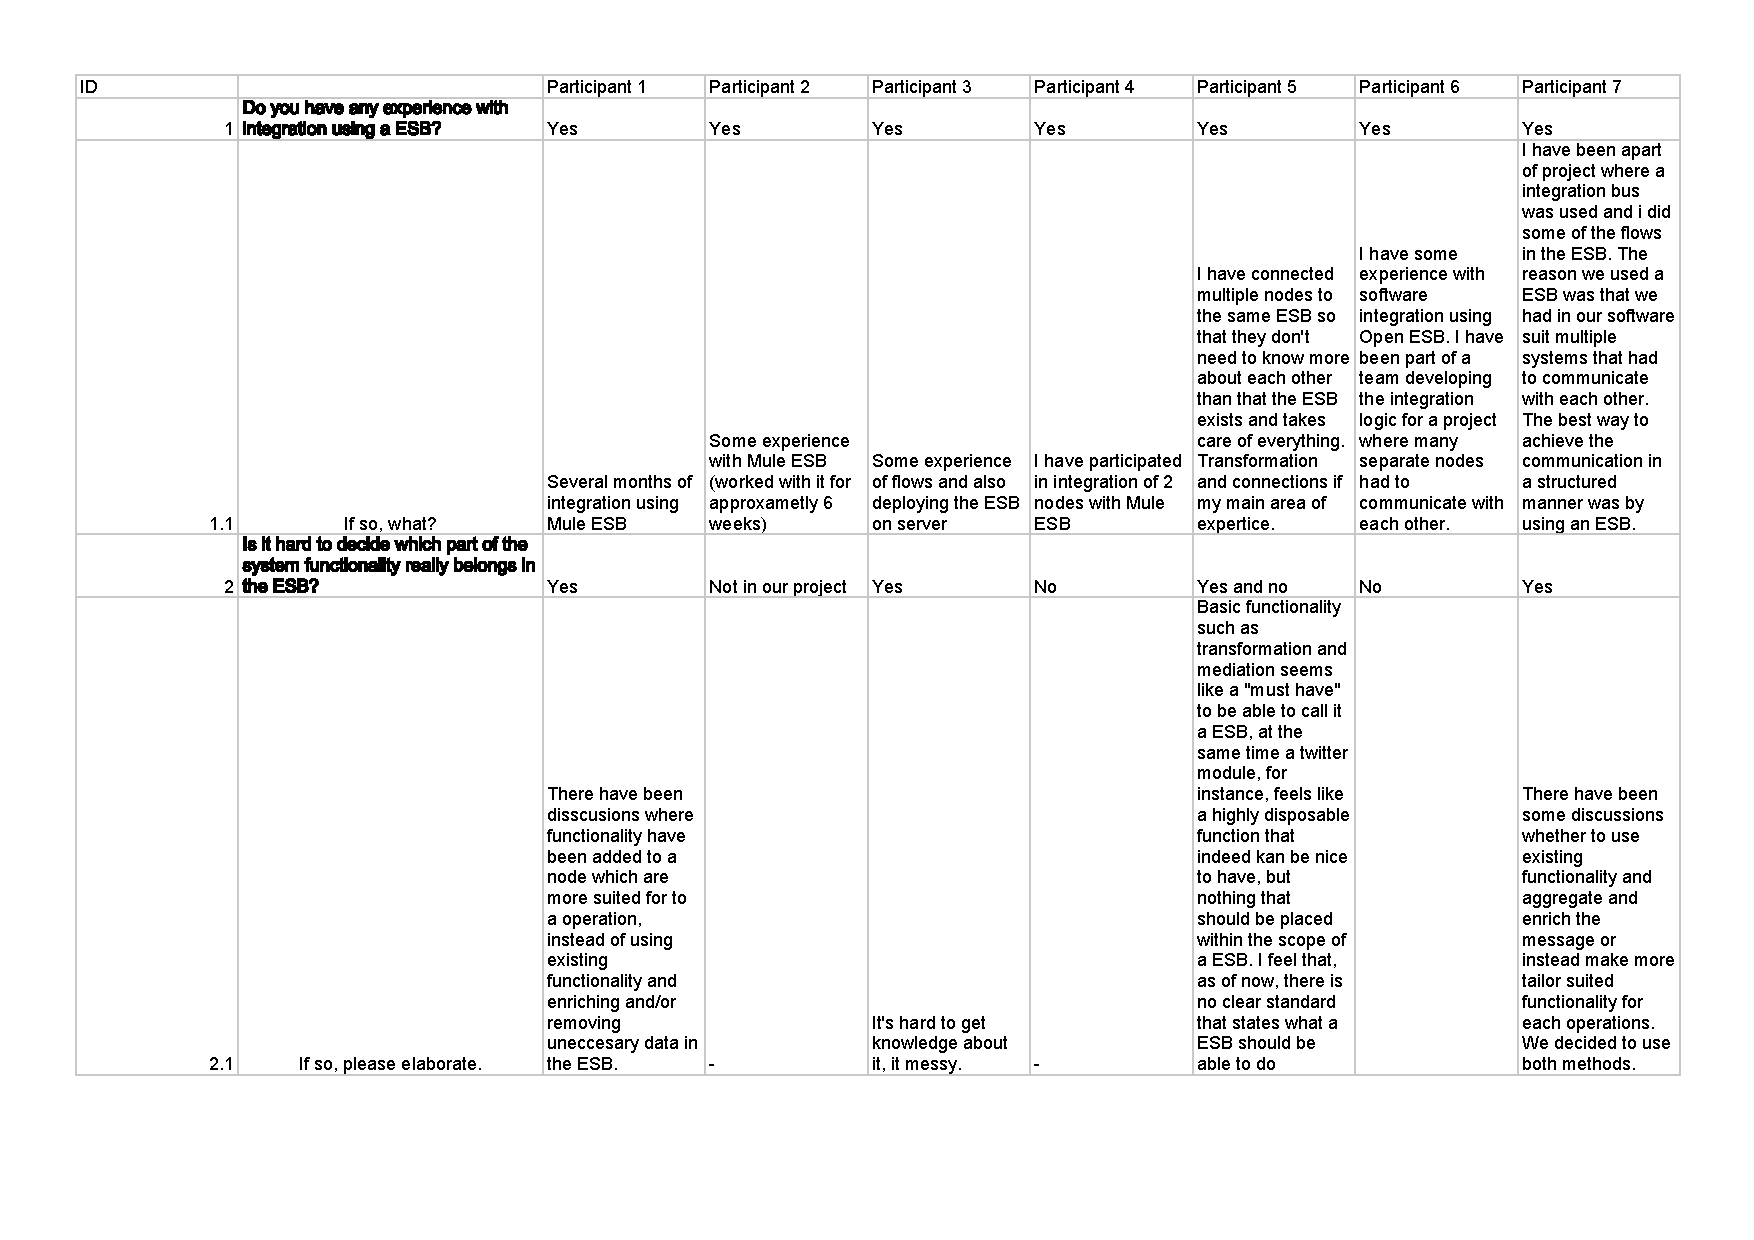
\includepdf[pages={1-5}]{appendix-a.pdf}

\end{document}